\section{Introduction}

\begin{figure}
    \centering
    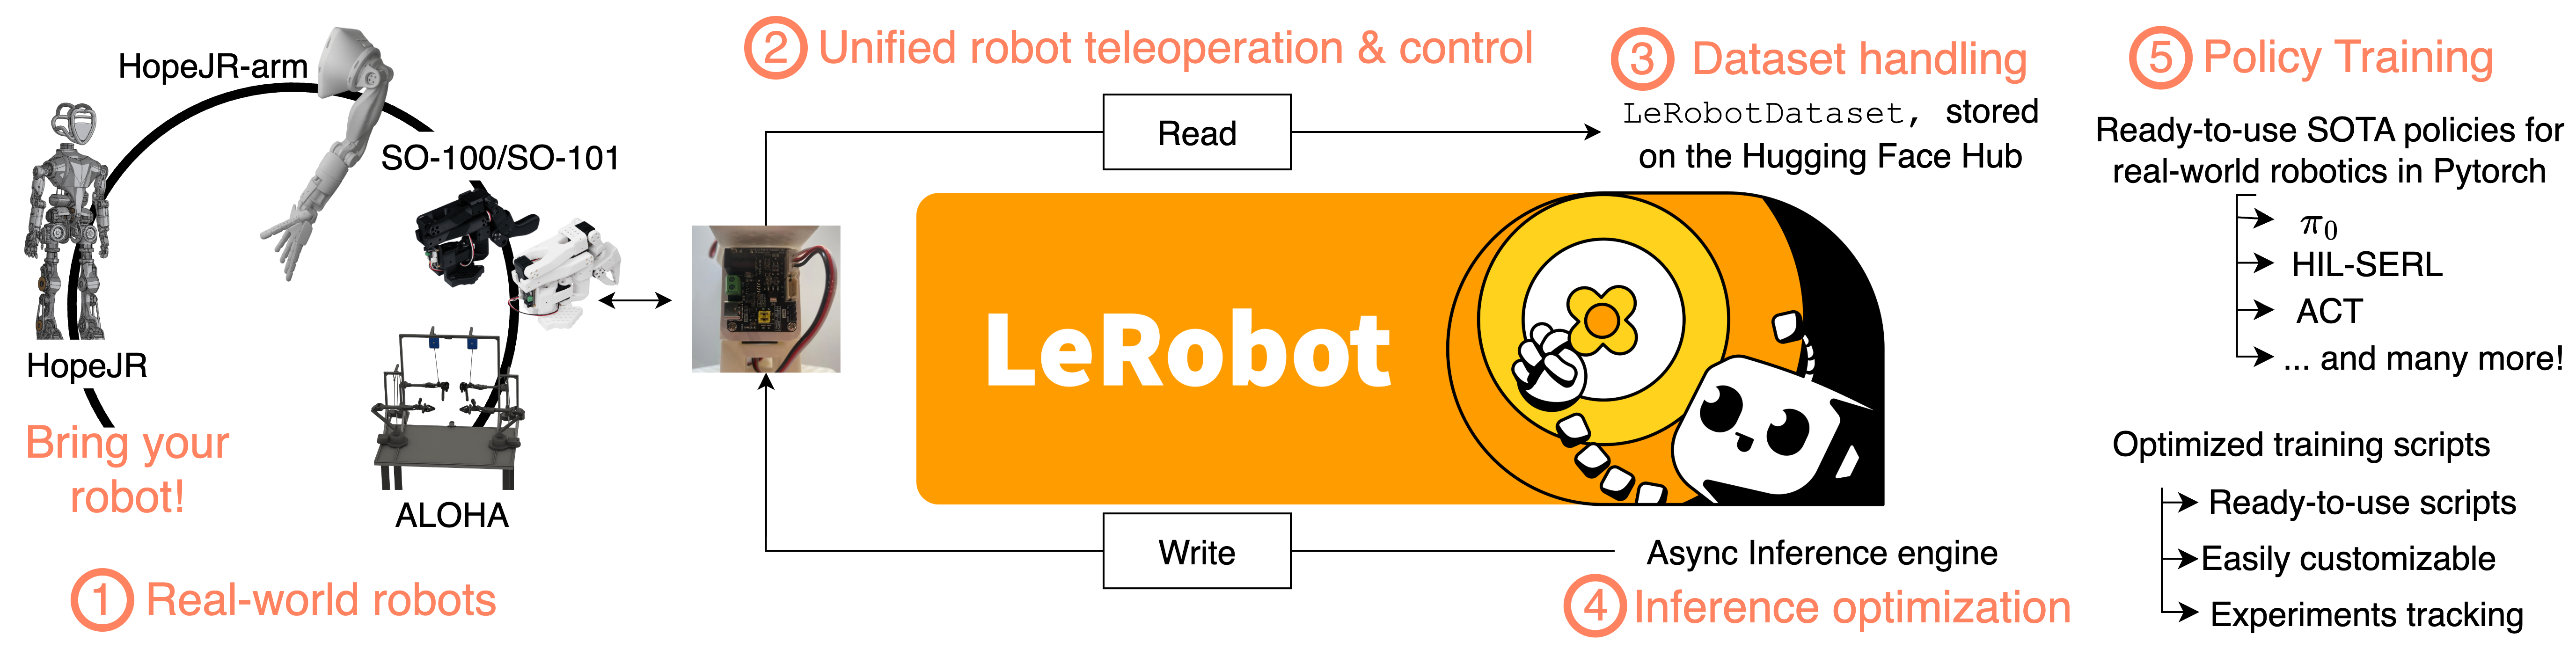
\includegraphics[width=\linewidth]{figures/ch1/ch1-lerobot-figure1.png}
    \caption{\lerobot \ is the open-source library for end-to-end robotics developed by Hugging Face. The library is vertically integrated on the entire robotics stack, supporting low-level control of real-world robot devices, advanced data and inference optimizations, as well as  SOTA robot learning methods ported in pure Pytorch.}
    \label{fig:figure1}
\end{figure}

Autonomous robotics holds the premise of relieving humans from repetitive, tiring or dangerous manual tasks. 
Consequently, the field of robotics has been widely studied since its first inception in the 1950s.
Lately, advancements in Machine Learning (ML) have sparked the development of a relatively new class of methods used to tackle robotics problems, leveraging large amounts of computation and data rather than human expertise and modeling to develop autonomous systems.

Robotics in 2025 sits is increasingly moving away from classical model-based control paradigm, embracing the advancements made in ML, thus unlocking (1) monolithic perception-to-action action pipelines and (2) multi-modal data-driven feature extraction strategies, together with (3) reduced reliance on precise models of the world and (4) a better positioning to benefit from the growing availability of robotics data openly available.
While central problems in manipulation, locomotion and whole-body control demand knowledge of rigid-body dynamics, contact modeling, planning under uncertainty, recent results seem to indicate learning can prove as effective as explicit modeling, sparking interest in the field of \emph{robot learning}.
This interest can be largely justified considering the significant challenges related to deriving accurate models of robot-environment interactions.
Also, because end-to-end learning on large and increasing amounts of data produced \emph{foundation models} capable to semantically reason over multiple input modalities (images, text, audio, etc.), deriving methods for robotics based on learning seems particularly promising, given the current trends related to the growth of openly available datasets.

At its core, robotics is also an inherently multi-disciplinary field, to the very least considering the diverse skills required in terms of \emph{software} and \emph{hardware}.
Integrating learning-based techniques increases the heterogeneity of skills needed to tackle robotics, whether in applications or research.
\lerobot is an open-source library end-to-end integrated with the entire robotics stack.
With a strong focus on accessible, real-world robots, \highlight{(1) \lerobot supports many, openly available, robotic platforms} for manipulation, locomotion and even whole-body control. 
\lerobot's \highlight{(2) unified, low-level approach to reading/writing robot configurations} also allows to extend support for other robots relatively easily. 
The library also supports \highlight{(3) a native robotics dataset's format}---\texttt{LeRobotDataset}---that is used to efficiently share datasets. 
\lerobot also supports many state-of-the-art (SOTA) algorithms in robot learning---Reinforcement Learning (RL) and Behavioral Cloning (BC)---with efficient implementations in Pytorch and extended support to experimentation and experiments tracking.
Lastly, \lerobot defines a custom, optimized inference stack for robotic policies decoupling action planning from action execution, proving effective in guaranteeing more adaptability at runtime.

This tutorial serves the double purpose of providing useful references for the science and practical use of common robot learning techniques.
To this aim, we strike to provide rigorous yet concise overviews of the core concepts behind the techniques presented, paired with practical examples of how to use these in applications, for practitioners and researchers in the field of robot learning.
This tutorial is structured as follows:
\begin{itemize}
\item Section~\ref{sec:classical} reviews classical robotics foundations, introducing the limitations of dynamics-based approaches to robotics.
\item Section~\ref{sec:learning} elaborates on the limitations of dynamics-based methods, and introduces learning-based techniques, their upsides and potential limitations.
\item Section~\ref{sec:single} further describes robot learning techniques that aim at solving single tasks learning from specific expert demonstrations.
\item Section~\ref{sec:multi} presents recent contributions towards generalist models for robotics applications learning from large corpora of multi-robot multi-task data.
\item Lastly, Section~\ref{sec:extensions} covers emerging directions in robot learning research, introducing recent works in post-training techniques for robotics foundation models.
\end{itemize}

Lastly, we complement our presentation of the most common and recent approaches in robot learning with practical code implementations using \lerobot.

% If time permits.
% \subsection{The \textit{LeRobotDataset} Format for Robotics Datasets}
% Structure of the dataset object
% Features stored

% \subsubsection{Code Example: Forwarding Batches of a (Streaming) Dataset}
